\documentclass[12pt]{article}
	
\title{CSC 320 - Worksheet 2}
\author{Nadeem Abdul Hamid}
\date{January 16, 2024}  


\usepackage[margin=1in]{geometry}		% For setting margins
\usepackage{amsmath}				% For Math
\usepackage{amsthm}
\usepackage{fancyhdr}				% For fancy header/footer
\usepackage{graphicx}				% For including figure/image
\usepackage{cancel}					% To use the slash to cancel out stuff in work
\usepackage[shortlabels]{enumitem}
\usepackage{hyperref}
\usepackage{jigsaw}

\usepackage{algorithm,caption}
\usepackage{algpseudocodex}
% docs: https://ctan.math.washington.edu/tex-archive/macros/latex/contrib/algpseudocodex/algpseudocodex.pdf


%%%%%%%%%%%%%%%%%%%%%%
% Set up fancy header/footer
% taken from https://www.overleaf.com/latex/templates/homework-template/yvgnmrbywwnp
\makeatletter    % for \@ in \@title
\pagestyle{fancy}
\fancyhead[LO,L]{\@author}
\fancyhead[CO,C]{\@title}
\fancyhead[RO,R]{\@date}
\fancyfoot[LO,L]{}
\fancyfoot[CO,C]{\thepage}
\fancyfoot[RO,R]{}
\renewcommand{\headrulewidth}{0.4pt}
\renewcommand{\footrulewidth}{0.4pt}
\makeatother    % restore
%%%%%%%%%%%%%%%%%%%%%%


%%%%%%%%%%%%%%%%%%%%%%
% from: https://tex.stackexchange.com/questions/14667/does-latex-define-a-semantic-equivalent-of-textbf
\makeatletter
\newcommand{\strong}[1]{\@strong{#1}}
\newcommand{\@@strong}[1]{\textbf{\let\@strong\@@@strong#1}}
\newcommand{\@@@strong}[1]{\textnormal{\let\@strong\@@strong#1}}
\let\@strong\@@strong
\makeatother
%%%%%%%%%%%%%%%%%%%%%%


\newcommand{\emptybox}[2][\textwidth]{%
  \begingroup
  \setlength{\fboxsep}{-\fboxrule}%
  \noindent\framebox[#1]{\rule{0pt}{#2}}%
  \endgroup
}

\newtheorem{theorem}{Theorem}
\newtheorem{lemma}{Lemma}


\begin{document}

\section{Analysis Framework; Asymptotic notation; Analysis of non-recursive algorithms}

\subsection{Input size measures}
For each of the following algorithms, indicate (i) a natural size metric for its inputs, (ii) its basic operation, and (iii) whether the basic operation count can be different for inputs of the same size:

\begin{enumerate}[a.]
    \item Computing the sum of $n$ numbers \vspace{.7in}
    \item Computing $n!$ \vspace{.7in}
    \item Finding the largest element in a list of $n$ numbers \vspace{.75in}
    \item Euclid’s algorithm \vspace{.75in}
    \item Sieve of Eratosthenes \vspace{.75in}
    \item Pen-and-pencil algorithm for multiplying two n-digit decimal integers \vspace{.75in}
\end{enumerate}


\clearpage
\subsection{Sequential search}

Use the most appropriate notation among $O$, $\Theta$, $\Omega$ to indicate the time efficiency class of sequential search:
\begin{enumerate}[a.]
    \item in the worst case.
    \item in the best case.
    \item in the average case.
\end{enumerate}

\vspace{3in}


Consider a variation of sequential search that scans a list to return the number of occurrences of a given search key in the list. Does its efficiency differ from the efficiency of classic sequential search?

\vspace{2in}

\clearpage
\subsection{Asymptotic notation}
For each of the following functions, indicate the class $\Theta(g(n))$ the function belongs to. (Use the simplest $g(n)$ possible in your answers.) Prove your assertions.

\begin{enumerate}[a.]
    \item $(n^2 + 1)^{10}$
    \item $\sqrt{10n^2 + 7n + 3}$
    \item $2n\cdot\textrm{lg}(n + 2)^2 + (n+2)^2 \textrm{lg}(\frac{n}{2})$
    \item $2^{n+1} + 3^{n-1}$
    \item $\lfloor\log_2 n\rfloor$
\end{enumerate}


\clearpage
\subsection{Analysis of iterative algorithm}

Consider the following algorithm:\\~

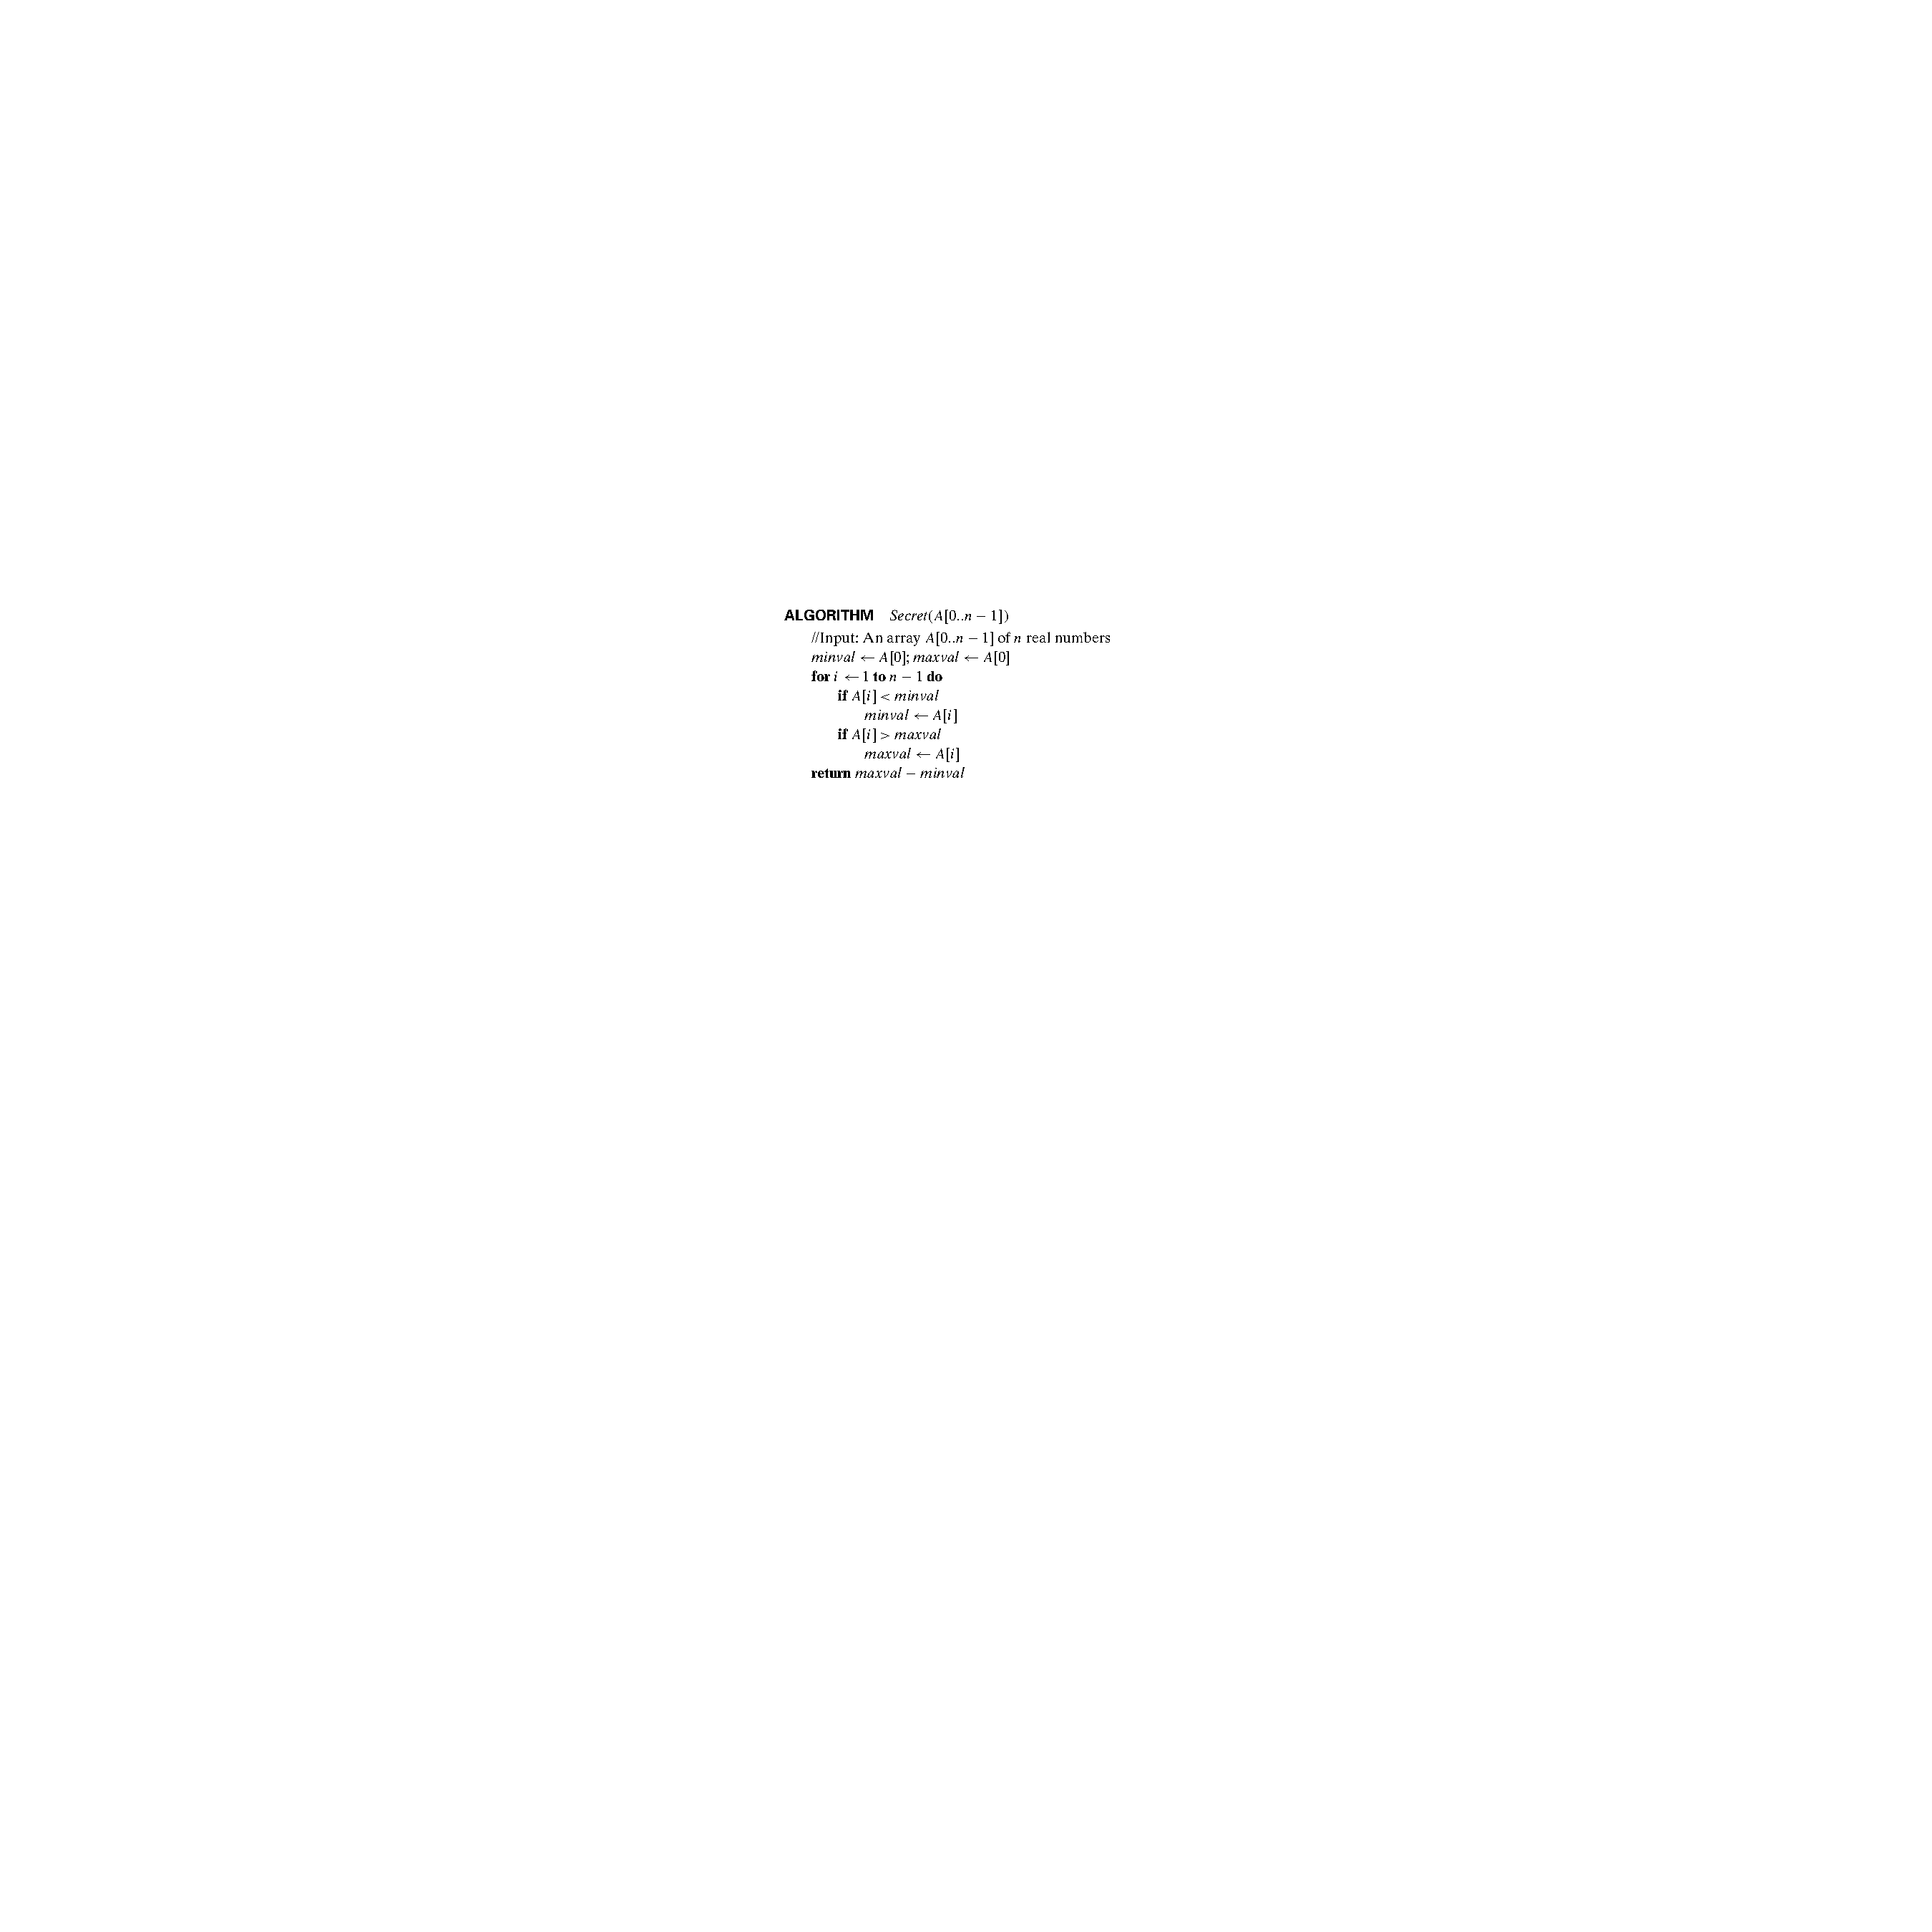
\includegraphics{w02-alg.pdf}

\begin{enumerate}[a.]
    \item What does this algorithm compute?
    \item What is its basic operation?
    \item How many times is the basic operation executed?
    \item What is the efficiency class of this algorithm?
    \item Suggest an improvement, or a better algorithm altogether, and indicate its efficiency class. If you cannot do it, try to prove that, in fact, it cannot be done.
\end{enumerate}

\end{document}



